\documentclass[]{article}
\usepackage{lmodern}
\usepackage{amssymb,amsmath}
\usepackage{ifxetex,ifluatex}
\usepackage{fixltx2e} % provides \textsubscript
\ifnum 0\ifxetex 1\fi\ifluatex 1\fi=0 % if pdftex
  \usepackage[T1]{fontenc}
  \usepackage[utf8]{inputenc}
\else % if luatex or xelatex
  \ifxetex
    \usepackage{mathspec}
  \else
    \usepackage{fontspec}
  \fi
  \defaultfontfeatures{Ligatures=TeX,Scale=MatchLowercase}
\fi
% use upquote if available, for straight quotes in verbatim environments
\IfFileExists{upquote.sty}{\usepackage{upquote}}{}
% use microtype if available
\IfFileExists{microtype.sty}{%
\usepackage{microtype}
\UseMicrotypeSet[protrusion]{basicmath} % disable protrusion for tt fonts
}{}
\usepackage[margin=1in]{geometry}
\usepackage{hyperref}
\hypersetup{unicode=true,
            pdfborder={0 0 0},
            breaklinks=true}
\urlstyle{same}  % don't use monospace font for urls
\usepackage{graphicx,grffile}
\makeatletter
\def\maxwidth{\ifdim\Gin@nat@width>\linewidth\linewidth\else\Gin@nat@width\fi}
\def\maxheight{\ifdim\Gin@nat@height>\textheight\textheight\else\Gin@nat@height\fi}
\makeatother
% Scale images if necessary, so that they will not overflow the page
% margins by default, and it is still possible to overwrite the defaults
% using explicit options in \includegraphics[width, height, ...]{}
\setkeys{Gin}{width=\maxwidth,height=\maxheight,keepaspectratio}
\IfFileExists{parskip.sty}{%
\usepackage{parskip}
}{% else
\setlength{\parindent}{0pt}
\setlength{\parskip}{6pt plus 2pt minus 1pt}
}
\setlength{\emergencystretch}{3em}  % prevent overfull lines
\providecommand{\tightlist}{%
  \setlength{\itemsep}{0pt}\setlength{\parskip}{0pt}}
\setcounter{secnumdepth}{0}
% Redefines (sub)paragraphs to behave more like sections
\ifx\paragraph\undefined\else
\let\oldparagraph\paragraph
\renewcommand{\paragraph}[1]{\oldparagraph{#1}\mbox{}}
\fi
\ifx\subparagraph\undefined\else
\let\oldsubparagraph\subparagraph
\renewcommand{\subparagraph}[1]{\oldsubparagraph{#1}\mbox{}}
\fi

%%% Use protect on footnotes to avoid problems with footnotes in titles
\let\rmarkdownfootnote\footnote%
\def\footnote{\protect\rmarkdownfootnote}

%%% Change title format to be more compact
\usepackage{titling}

% Create subtitle command for use in maketitle
\newcommand{\subtitle}[1]{
  \posttitle{
    \begin{center}\large#1\end{center}
    }
}

\setlength{\droptitle}{-2em}

  \title{}
    \pretitle{\vspace{\droptitle}}
  \posttitle{}
    \author{}
    \preauthor{}\postauthor{}
    \date{}
    \predate{}\postdate{}
  

\begin{document}

\begin{center}\rule{0.5\linewidth}{\linethickness}\end{center}

\section{March, 2019: Dr.~Susan
Sangha}\label{march-2019-dr.susan-sangha}

\begin{figure}
\centering
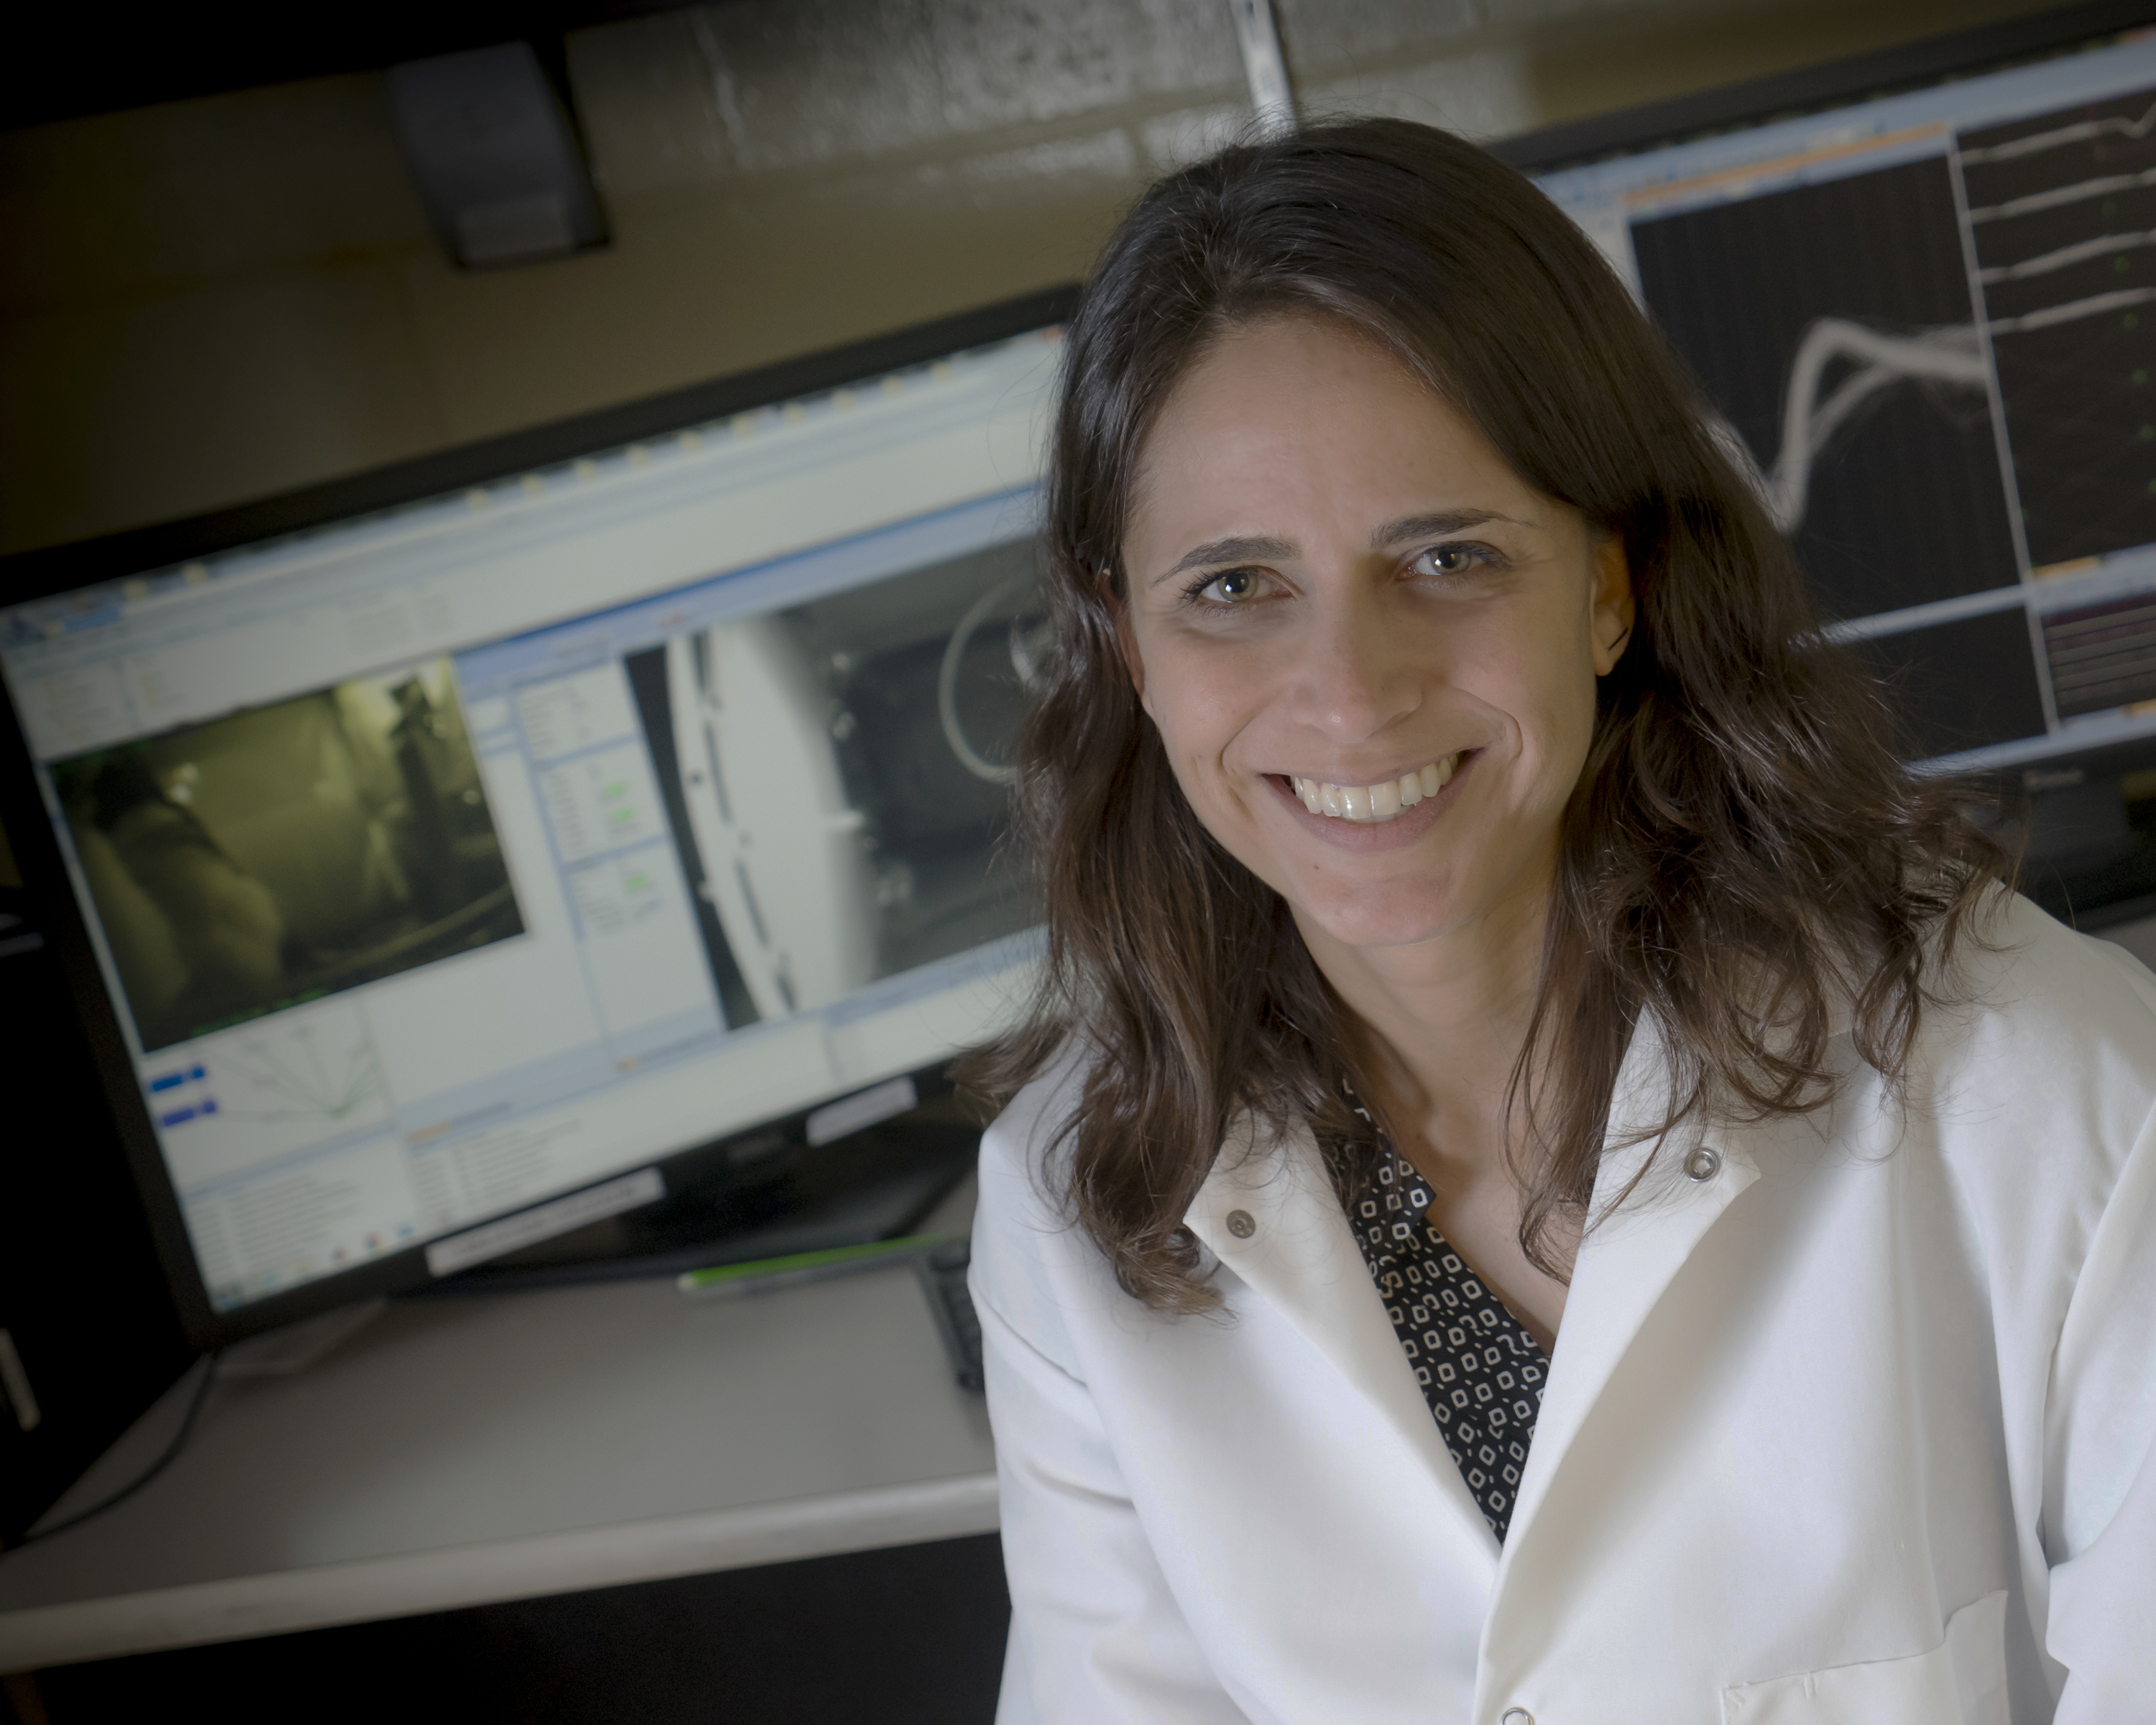
\includegraphics{./photos/Sangha_lab.jpg}
\caption{Dr.~Sangha in her lab at Purdue University.}
\end{figure}

Dr.~Susan Sangha is an Assistant Professor of Psychological Sciences at
the Purdue University Institute for Integrative Neuroscience. Before
starting her own lab in Purdue, Dr.~Sangha received her PhD from the
University of Calgary in the lab of Dr.~Ken Lukowiak and completed
separate postdoctoral fellowships under Dr.~Hans-Christian Pape and
Dr.~Patricia Janak. Dr.~Sangha and her students combine elegant behavior
with in vivo single-unit electrophysiology and pharmacogenetics to
understand how the brain changes during fear, safety, and reward cue
learning.

\begin{center}\rule{0.5\linewidth}{\linethickness}\end{center}

\subsubsection{\texorpdfstring{\textbf{What project are you currently
most excited about in your
lab?}}{What project are you currently most excited about in your lab?}}\label{what-project-are-you-currently-most-excited-about-in-your-lab}

Right now, we have some exciting neural data from the PFC collected in
freely behaving rats during our safety learning task. At the single
neuron level, we are seeing many neurons in the infralimbic cortex
responding to a learned safety cue while fear behavior is being
suppressed.

\subsubsection{\texorpdfstring{\textbf{What challenges, if any, have you
experienced as a woman in
learning?}}{What challenges, if any, have you experienced as a woman in learning?}}\label{what-challenges-if-any-have-you-experienced-as-a-woman-in-learning}

I feel like I have been overall quite lucky to have had really
supportive mentors, both male and female, throughout my career. However,
when I got my faculty position and was the `boss' of the lab and
classroom, it appeared to me I was not getting the same level of respect
from students, in the classroom and in the lab, as a new male PI would.

\subsubsection{\texorpdfstring{\textbf{What advice would you give
yourself 10 years
ago?}}{What advice would you give yourself 10 years ago?}}\label{what-advice-would-you-give-yourself-10-years-ago}

That would be 2009, when I finished my first postdoc and was starting my
second postdoc. The thing I did right was take a chance and start my
line of research on safety learning. The advice I would give myself
would probably be ``ok, breathe, relax, it'll all be fine''. I was too
stressed about getting the faculty position. I obviously succeeded in
getting one, but life would have been fine if I didn't.

\subsubsection{\texorpdfstring{\textbf{What's your favorite
pie?}}{What's your favorite pie?}}\label{whats-your-favorite-pie}

I don't like pie. I do like chocolate cake though.

\subsubsection{\texorpdfstring{\textbf{What's your favorite
season?}}{What's your favorite season?}}\label{whats-your-favorite-season}

Fall, I go gaga over colorful fall foliage.

\subsubsection{\texorpdfstring{\textbf{What's your ideal Saturday out of
the
office?}}{What's your ideal Saturday out of the office?}}\label{whats-your-ideal-saturday-out-of-the-office}

Being outside, taking photos and playing with my dog. I don't live near
mountains anymore but a hike in the mountains would be a perfect
Saturday.

\subsubsection{\texorpdfstring{\textbf{What do you love about the
Pavlovian
Society?}}{What do you love about the Pavlovian Society?}}\label{what-do-you-love-about-the-pavlovian-society}

Over the years, it has become to me an interactive and supportive
community filled with other learning nerds.

\begin{figure}
\centering
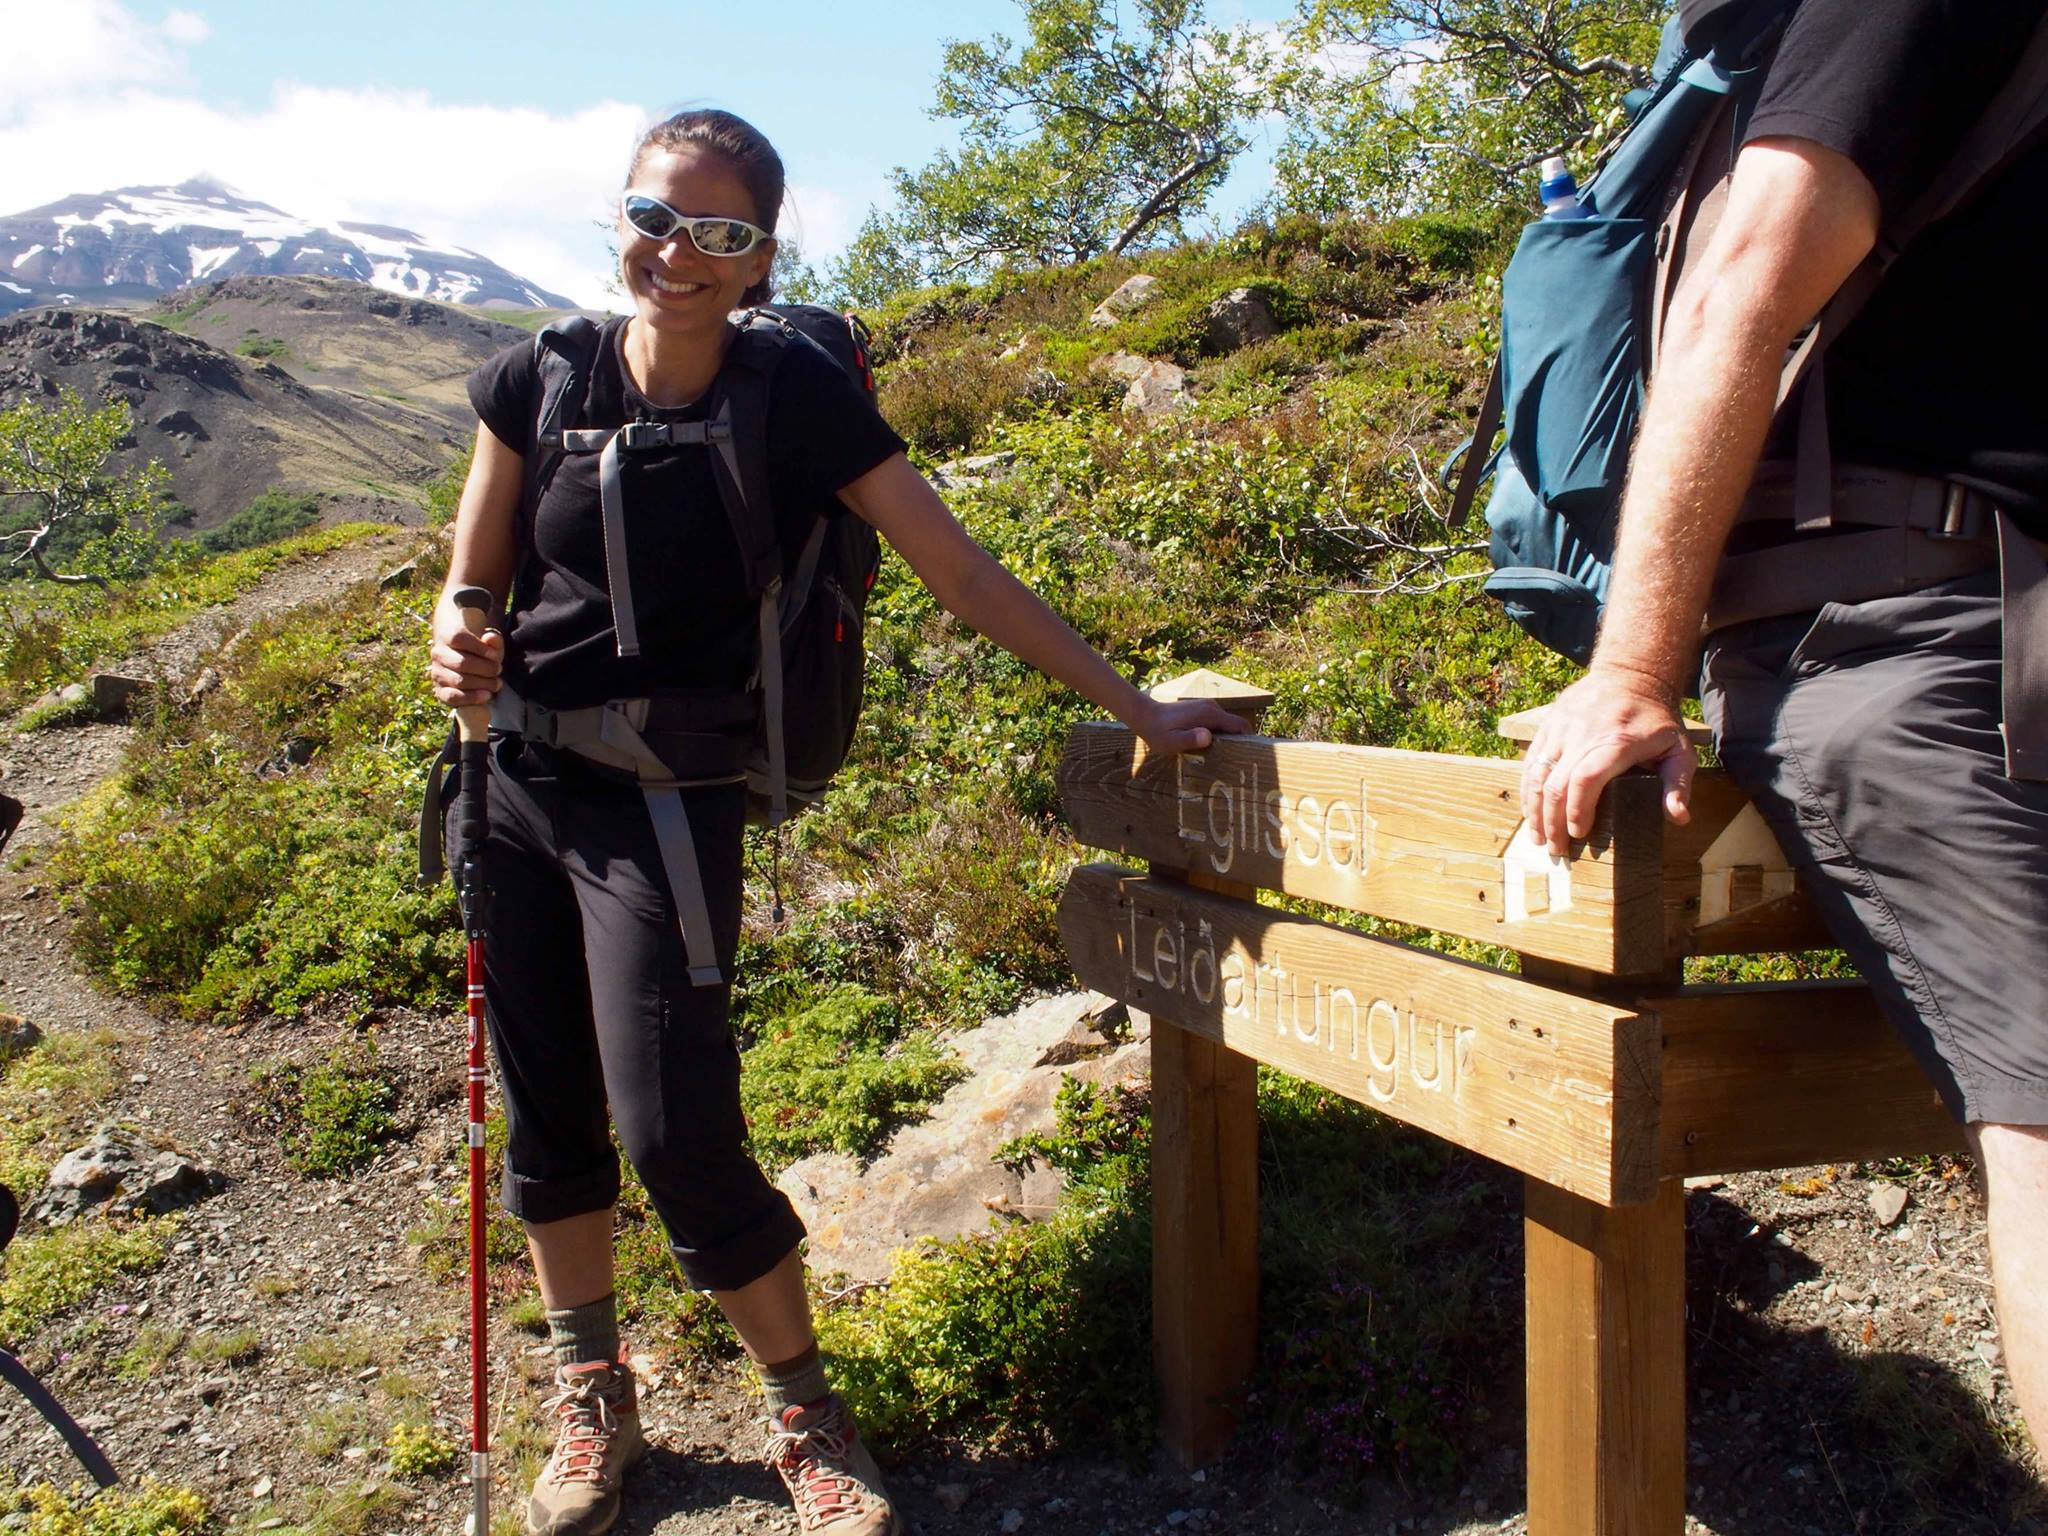
\includegraphics{./photos/Sangha_iceland.jpg}
\caption{Dr.~Sangha hiking in Iceland. ``This was the first time I left
the lab for an extended period of time. I had no cell or internet
service for 10 days; I was nervous to do it, but the lab did just
fine!''}
\end{figure}

\begin{center}\rule{0.5\linewidth}{\linethickness}\end{center}

This page was developed by Peter Euclide
(\href{mailto:peter.euclide@uwsp.edu}{\nolinkurl{peter.euclide@uwsp.edu}})
and maintained by Sydney Trask
(\href{mailto:trask@uwm.edu}{\nolinkurl{trask@uwm.edu}}). A complete
record of the Pavolvian Society's Featured Faculty series can be found
at \url{https://sydneytrask.github.io/Featured_Faculty.html}


\end{document}
